\documentclass[11pt,a4paper]{article}
\usepackage[margin=22mm]{geometry}
\usepackage[T1]{fontenc}
\usepackage{lmodern,amsmath,amssymb,booktabs,array,graphicx,tikz,listings,xcolor,hyperref}
\usetikzlibrary{arrows.meta,positioning,shapes.geometric,calc}
\hypersetup{pdftitle={Cedar-8f2c student reference},pdfauthor={Cedar-8f2c},colorlinks=true,linkcolor=blue,urlcolor=blue}
\lstset{basicstyle=\ttfamily\small,breaklines=true,columns=fullflexible,frame=single}
\newcommand{\bits}[1]{\texttt{#1}}
\newcommand{\reference}{\noindent\textbf{Student reference.} This is an anonymous, editable reconstruction of the supplied student report. It preserves the student's approach and reported results. Editorial verification notes and assignment clarifications are labeled separately. It is not a newly corrected solution or a claim of full fault coverage. The accompanying anonymized PDF preserves the original evidence.\par}
\title{Homework 1: BIST and BISR\\Student reference}
\author{Cedar-8f2c}
\date{}
\begin{document}
\maketitle
\reference

\section{Assignment and supplementary requirements}
The assignment asks for a 16-bit ripple carry adder with built-in self-test (BIST), followed by a repairable version with one spare full adder. The BIST should detect single cell faults. The repair design should locate a faulty full adder and restore normal arithmetic.
The supplementary instructions require test-mode patterns to originate inside the BIST. An external testbench may supply operands only in normal mode. Fault injection must support every one of the 16 full-adder positions, with one faulty cell at a time. The report should show normal arithmetic, a fault changing the result, detection in test mode, and arithmetic after repair. A representative waveform is permitted, but the intended coverage still applies to every supported fault.

\section{Part 1: BIST architecture}
The student places a pattern source and response comparator in front of a 16-bit ripple carry adder. The signals \bits{Test}, \bits{En}, \bits{Clk}, and \bits{Rst} select normal operation or the embedded pattern sequence. The 17-bit response includes all sum bits and the final carry. The signal \bits{P\_F} is zero for pass and becomes one after a mismatch.
\begin{figure}[ht]\centering
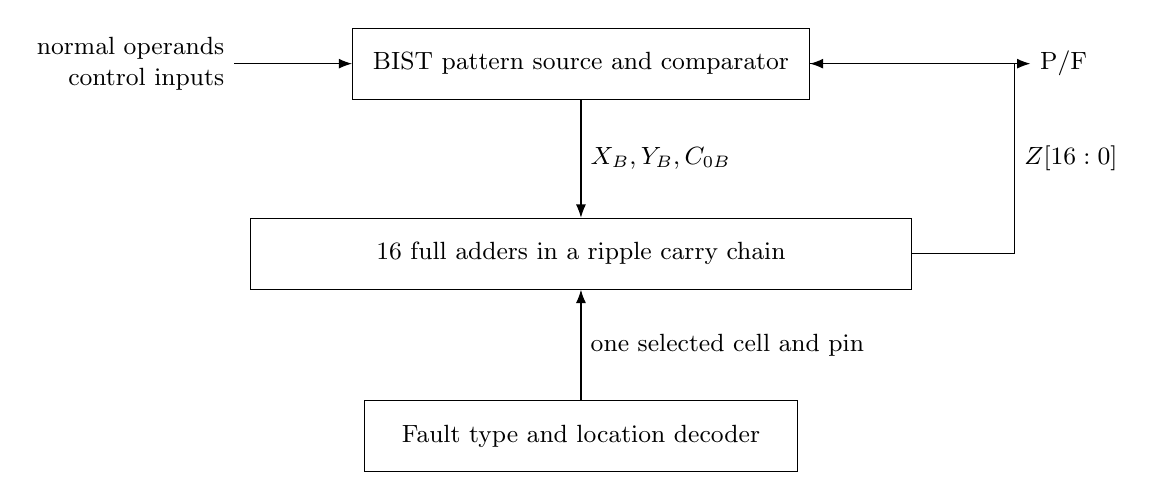
\begin{tikzpicture}[>=Latex,every node/.style={font=\small},b/.style={draw,minimum height=9mm,align=center}]
\node[b,minimum width=58mm] (bist) {BIST pattern source and comparator};
\node[b,below=15mm of bist,minimum width=84mm] (adder) {16 full adders in a ripple carry chain};
\node[b,below=14mm of adder,minimum width=55mm] (fault) {Fault type and location decoder};
\draw[->] (bist) -- node[right] {$X_B,Y_B,C_{0B}$} (adder);
\draw[->] (adder.east) -- ++(13mm,0) |- node[pos=.25,right] {$Z[16:0]$} (bist.east);
\draw[->] (fault) -- node[right] {one selected cell and pin} (adder);
\draw[<-] (bist.west) -- ++(-15mm,0) node[left,align=right] {normal operands\\control inputs};
\draw[->] (bist.east) -- ++(28mm,0) node[right] {P/F};
\end{tikzpicture}
\caption{Editable reconstruction of the source presentation's BIST architecture.}
\end{figure}

\subsection{Pattern selection and comparison}
Normal mode forwards the external operands and carry input. Test mode with \bits{En=0} holds the embedded operands. With \bits{En=1}, the design alternates all-zero and all-one operands, including the carry input, and compares the response with the expected value. The implementation pipelines the comparison. Reset clears the failure flag and pattern counters.
\begin{center}\begin{tabular}{lll}
\toprule Mode & Operand source & Action\\
\midrule
Test=0 & External $X,Y,C_0$ & Normal arithmetic\\
Test=1, En=0 & Held embedded values & Hold sequence\\
Test=1, En=1 & Alternating embedded patterns & Compare response\\
Mismatch & -- & Set sticky P/F failure flag\\
\bottomrule\end{tabular}\end{center}

\subsection{Fault model and pattern argument}
The student uses ten pin stuck-at faults per full adder:
\[
\{X/0,X/1,Y/0,Y/1,C_{\rm in}/0,C_{\rm in}/1,S/0,S/1,C_{\rm out}/0,C_{\rm out}/1\}.
\]
The source report gives this complete sum-output table. A fault column forces the named pin to the stated value.
\begin{center}\scriptsize\begin{tabular}{ccc|c|cccccccc}
\toprule
$X$&$Y$&$C_{\rm in}$&$S$&$X/0$&$X/1$&$Y/0$&$Y/1$&$C_{\rm in}/0$&$C_{\rm in}/1$&$S/0$&$S/1$\\
\midrule
0&0&0&0&0&1&0&1&0&1&0&1\\
0&0&1&1&1&0&1&0&0&1&0&1\\
0&1&0&1&1&0&0&1&1&0&0&1\\
0&1&1&0&0&1&1&0&1&0&0&1\\
1&0&0&1&0&1&1&0&1&0&0&1\\
1&0&1&0&1&0&0&1&1&0&0&1\\
1&1&0&0&1&0&1&0&0&1&0&1\\
1&1&1&1&0&1&0&1&0&1&0&1\\
\bottomrule\end{tabular}\end{center}
The report argues that $(0,0,0)$ detects the five stuck-at-one faults and $(1,1,1)$ detects the five stuck-at-zero faults when sum and carry are observed. For the whole adder these patterns become
\[
(X,Y,C_0)=(0,0,0),\qquad(65535,65535,1),
\]
with expected 17-bit responses $0$ and $131071$.
\paragraph{Editorial verification note.}
This argument concerns the ten stated pin stuck-at faults. General single-cell functional faults can alter an arbitrary truth-table entry. Two input combinations do not establish coverage of that broader model. The report's coverage claim therefore requires this qualification.

\subsection{Fault injection}
The four-bit \bits{Fault\_loc} chooses one of 16 full adders. The upper five bits of \bits{Fault\_type} select a pin, and bit zero gives its forced value.
\begin{center}\begin{tabular}{cl}
\toprule Fault\_type[5:1]&Selected pin\\\midrule
00000&No fault\\10000&$X$\\01000&$Y$\\00100&$C_{\rm in}$\\00010&$S$\\00001&$C_{\rm out}$\\
\bottomrule\end{tabular}\end{center}
Only one pin selection is intended at a time. Bit zero equal to zero means stuck-at-zero, while bit zero equal to one means stuck-at-one.

\subsection{Reported waveform example}
The report first demonstrates normal arithmetic. It injects a $Y$ stuck-at-zero fault at full adder 4. For $X=1300$, $Y=56$, and $C_0=1$, the correct result is $1357$ and the faulty result is $1341$. Entering test mode and enabling embedded patterns makes \bits{P\_F} become one.
\begin{center}\begin{tabular}{llll}
\toprule Stage&Test&Fault&Reported observation\\\midrule
Normal arithmetic&0&None&Correct sums\\
Injection&0&FA4, $Y/0$&$1357\longrightarrow1341$\\
Embedded test&1&FA4, $Y/0$&Mismatch, P/F=1\\
\bottomrule\end{tabular}\end{center}
This event table reconstructs the source waveform's explanation. It is not a new simulation trace.

\section{Part 2: BISR}
The design adds one spare full adder and inserts its sum and carry into the chain after locating a fault. It compares the observed response with the expected response:
\[
D=Z_{\rm compare}\oplus Z_{\rm correct}.
\]
A priority decoder examines $D$ from the least significant bit toward the most significant bit. The first nonzero bit selects the full adder to replace. A mismatch only in the final carry selects full adder 15.
\begin{figure}[ht]\centering
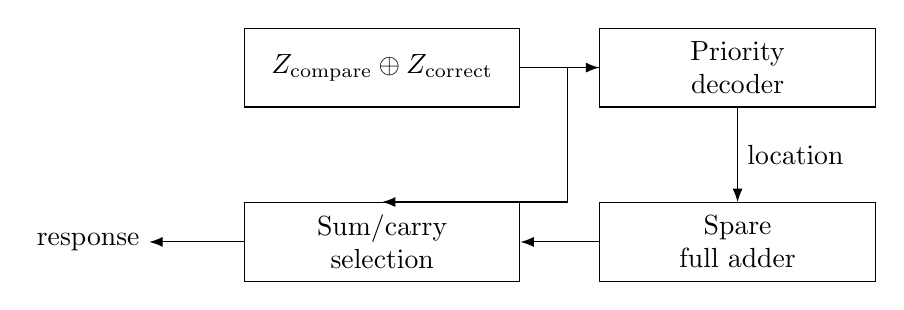
\begin{tikzpicture}[>=Latex,b/.style={draw,align=center,minimum width=35mm,minimum height=10mm}]
\node[b] (compare) {$Z_{\rm compare}\oplus Z_{\rm correct}$};
\node[b,right=10mm of compare] (decode) {Priority\\decoder};
\node[b,below=12mm of decode] (spare) {Spare\\full adder};
\node[b,left=10mm of spare] (mux) {Sum/carry\\selection};
\draw[->] (compare)--(decode);
\draw[->] (decode)--node[right] {location}(spare);
\draw[->] (spare)--(mux);
\draw[->] (decode.west)--++(-4mm,0)|-(mux.north);
\draw[->] (mux.west)--++(-12mm,0)node[left] {response};
\end{tikzpicture}
\caption{Editable reconstruction of the fault-location and spare-selection method.}
\end{figure}
Once failure is asserted, location-dependent logic sends the selected stage's original operands and incoming carry to the spare. It replaces that stage's sum and drives the next stage from the spare carry.
The source report shows excerpts of the \bits{casez} priority decoder and the replacement \bits{case} statement. The complete implementation is retained in the accompanying Verilog.

The final reported waveform repeats normal operation and injection, identifies the faulty location, and demonstrates correct arithmetic with the spare.
\paragraph{Editorial verification note.}
The first erroneous sum bit need not identify the physical source of every carry-output fault. Each stage and fault type requires directed testing. This reconstruction preserves the student's claim, while the repository's verification notes report observed limitations separately.

\section{Source selection}
The submitted \bits{hw1\_1.v}, \bits{hw1\_1\_tb.v}, \bits{hw1\_2.v}, and \bits{hw1\_2\_tb.v} are the primary set. A second top-level source copy is identical. Distinct files from two project source directories remain in separate legacy directories. Reused module names require separate compilation. Project files, generated simulation files, and caches are unnecessary.
\section{Repository verification}
Icarus Verilog 13.0 executed the retained RTL and the supplied testbenches. A separate testbench checks 100 normal operand combinations and all $16\times5\times2=160$ supported pin stuck-at injections. The BIST has no normal-arithmetic failures, keeps P/F zero on a good circuit, and detects all 160 injected faults under this sequence.
The BISR also detects all 160 injections, but its decoded location differs from the injected cell in 34 cases. After each test, a normal-mode calculation of $1300+56+1$ is checked. It returns an incorrect result for 37 of the 160 injections. These are observed limitations of the preserved reference, not edits to the student's submission. This directed test does not establish correctness for every post-repair operand or a general cell-functional fault model. The reproducible driver is \bits{verification/run\_checks.py} relative to the homework collection.
\end{document}
